\documentclass[11pt, a4paper]{report} % Classe: report (per capitoli) o article

% Pacchetti fondamentali
\usepackage[utf8]{inputenc} % Codifica caratteri
\usepackage[T1]{fontenc}    % Codifica font
\usepackage[italian]{babel} % Lingua
\usepackage{graphicx}       % Inserimento immagini
\usepackage{amsmath}        % Formule matematiche
\usepackage{hyperref} 
\usepackage{subcaption}
\usepackage{geometry}       % Margini
\usepackage{float}
\geometry{a4paper, margin=1in}
\usepackage{ragged2e}
\RaggedRight                % Rende tutto il documento allineato a sinistra


% Dati della relazione
\title{Relazione Progetto Business Intelligence Per i Servizi Finanziari 25/26}
\author{Luca Giani [909374]}
\date{\today}
\begin{document}

\maketitle % Crea il frontespizio
\tableofcontents % Indice automatico

\chapter{Introduzione}

\section{Titoli scelti}

I 6 titoli appartenenti all'indice S\&P 500 scelti per l'analisi sono stati:
\begin{enumerate}
    \item Settore Tecnologico: 
    \begin{itemize}
        \item NVIDIA (NVDA): leader nel settore dei semiconduttori e dell'intelligenza artificiale, con una forte crescita negli ultimi anni. È stata scelta visto il suo ruolo chiave nel'AI che è un settore in forte espansione, visto il rally che ha avuto negli ultimi anni e la recente notizia di 1 Trilione di ricavi cumulativi entro la fine del 2027.
        \item Microsoft (MSFT): gigante tecnologico con una vasta gamma di prodotti e servizi, tra cui software, cloud computing e intelligenza artificiale. È stato scelto proprio per la sua capcità di reinventarsi durante gli anni e rimanere per anni all'interno dei "magnificent-seven".
    \end{itemize}
        
    \item Settore Energetico: 
    \begin{itemize}
        \item ExxonMobil (XOM): azienda petrolifera leader mondiale, con una forte presenza in tutto il mondo. È stata scelta per la sua posizione di leadership nel settore energetico, essendo la compagnia americana con la maggiore capitalizzazione di mercato e perchè a differenza delle altre compagnie è più caute riguardo gli investimenti nelle energie rinnovabili.
        \item NextEra Energy (NEE): azienda energetica americana, con una forte presenza nel settore delle energie rinnovabili. È stata scelta per il suo orientamento verso le energie rinnovabili rispetto a ExxonMobil. 
    \end{itemize}

    Inoltre entrambi sono state scelte per analizzare i trend del settore energetico sia rinnovabile che quello dei combustibili fossili nei periodi di tensioni geopolitiche, come la guerra in Ucraina e Iran e per il trend di calo durante la pandemia, essendo il settore energetico quello più colpito, visto le diminuzione di domanda del petrolio.

    \item Settore Automobilistico: 
    \begin{itemize}
        \item Tesla (TSLA): azienda specializzata nella produzione di veicoli elettrici (EV). È stata scelta poichè nonostante l'intensificarsi della concorrenza da parte dei costruttori cinesi, Tesla sta mantenendo una posizione di rilievo agli investimenti per la creazione di robotaxi.
        \item General Motors (GM): azienda leader in America basata su veicoli a motore. È stata scelta per il suo obbiettivo annunciato di produrre solo veicoli elettrici entro il 2035.
    \end{itemize}
\end{enumerate}

\section{Funzioni utilizzate}
Le funzioni utilizzate per scaricare i dati sono:
\begin{itemize}
    \item \texttt{yfinance.download()}: per scaricare i dati storici dei prezzi delle azioni.
    \item \texttt{pandas.DataFrame}: per manipolare e analizzare i dati scaricati.
\end{itemize}

Ad esempio, è stato utilizzato \texttt{pandas.DataFrame.xs()} per dividere il DataFrame multilevel in più DataFrame, uno per ogni titolo.

\section{Breve Presentazione dei dati}
\begin{itemize}
    \item \textbf{NVIDIA (NVDA)}:
        Il titolo mostra una crescita esponenziale negli ultimi anni dovuta alla posizione di leadership nel settore dei semiconduttori e dell'intelligenza artificiale.
        \begin{figure}[H]
            \centering
            \begin{subfigure}{0.43\textwidth}
                \centering
                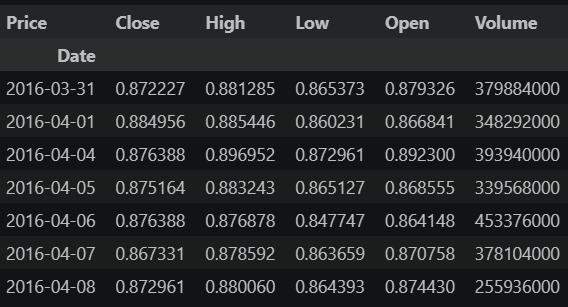
\includegraphics[width=\textwidth]{./images/NVDA_data_display.png}
                \caption{\texttt{DataFrame.head()}}
            \end{subfigure}
            \quad
            \begin{subfigure}{0.43\textwidth}
                \centering
                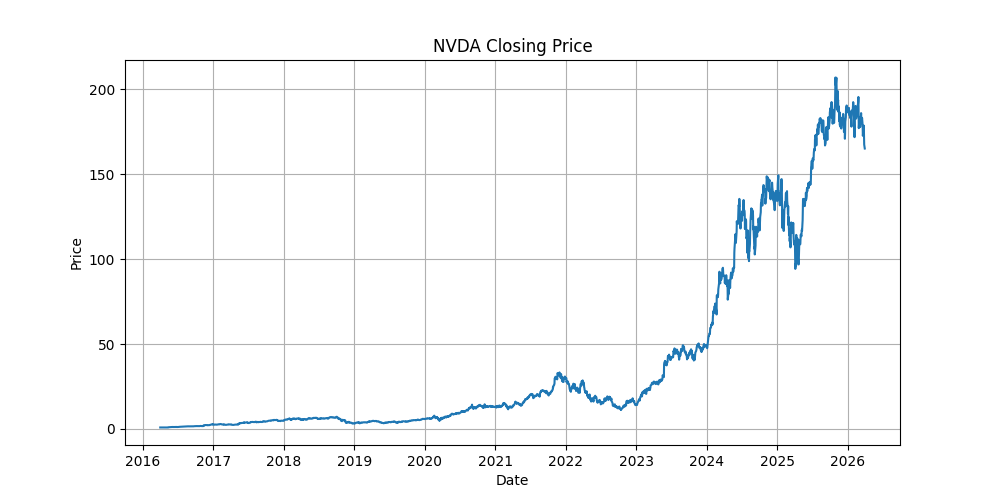
\includegraphics[width=\textwidth]{./images/NVDA_data_presentation.png}
                \caption{Prezzo di chiusura}
            \end{subfigure}
        \end{figure}
    \item \textbf{Microsoft (MSFT)}: 
        Il titolo mostra una crescita costante negli ultimi anni, principalmente a causa della sua leadership nel settore del software e dei servizi cloud.
        \begin{figure}[H]
            \centering
            \begin{subfigure}{0.43\textwidth}
                \centering
                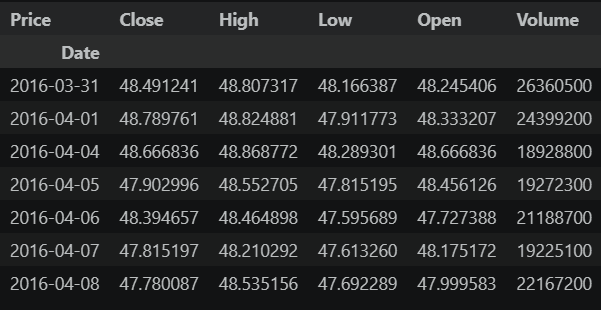
\includegraphics[width=\textwidth]{./images/MSFT_data_display.png}
                \caption{\texttt{DataFrame.head()}}
            \end{subfigure}
            \quad 
            \begin{subfigure}{0.43\textwidth}
                \centering
                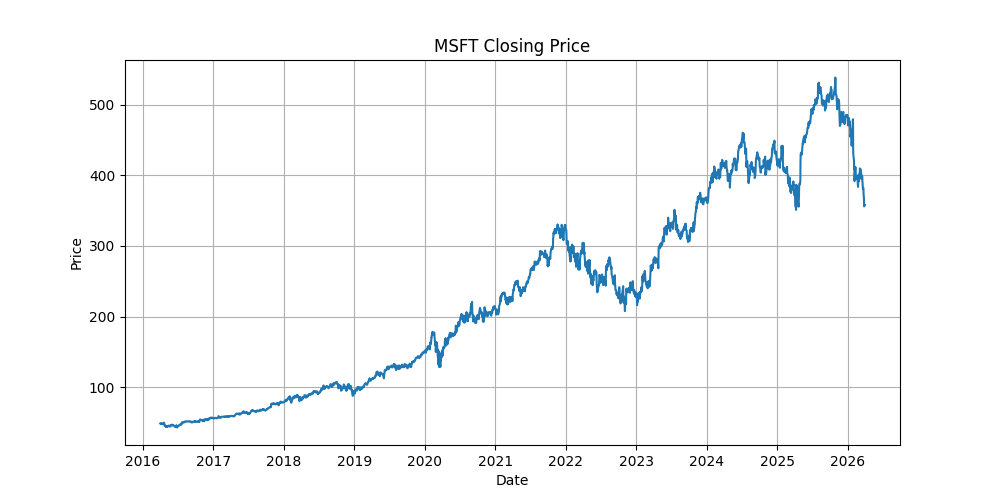
\includegraphics[width=\textwidth]{./images/MSFT_data_presentation.png}
                \caption{Prezzo di chiusura}
            \end{subfigure}
        \end{figure}
    \item \textbf{ExxonMobil (XOM)}: 
        Il titolo mostra una crescita variabile negli ultimi anni, influenzata dalle fluttuazioni dei prezzi del petrolio e dalle dinamiche del mercato energetico a sua volta influenzati dalle tensioni geopolitiche.
        \begin{figure}[H]
            \centering
            \begin{subfigure}{0.43\textwidth}
                \centering
                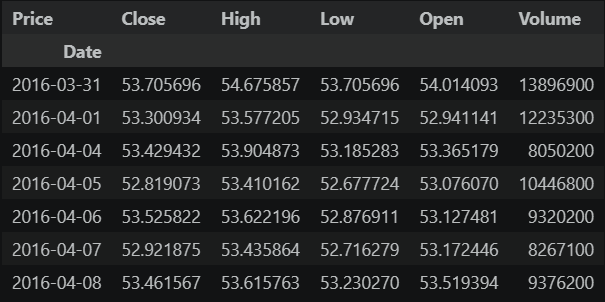
\includegraphics[width=\textwidth]{./images/XOM_data_display.png}
                \caption{\texttt{DataFrame.head()}}
            \end{subfigure}
            \quad
            \begin{subfigure}{0.43\textwidth}
                \centering
                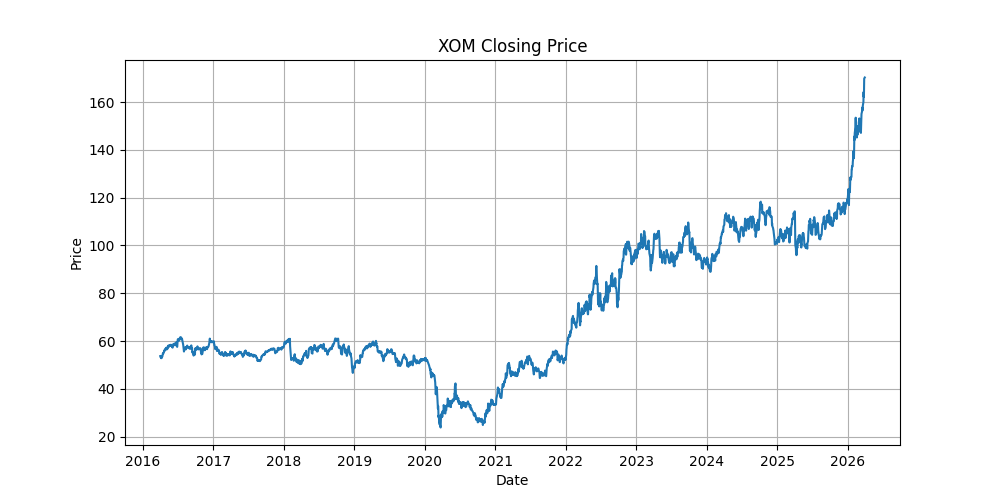
\includegraphics[width=\textwidth]{./images/XOM_data_presentation.png}
                \caption{Prezzo di chiusura}
            \end{subfigure}
        \end{figure}
    \item \textbf{NextEra Energy (NEE)}: 
        Il titolo mostra una crescita quasi costante, interrotta e poi ripresa da un periodo di calo.
        \begin{figure}[H]
            \centering
            \begin{subfigure}{0.43\textwidth}
                \centering
                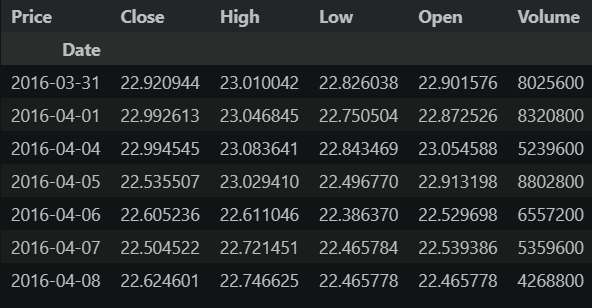
\includegraphics[width=\textwidth]{./images/NEE_data_display.png}
                \caption{\texttt{DataFrame.head()}}
            \end{subfigure}
            \quad 
            \begin{subfigure}{0.43\textwidth}
                \centering
                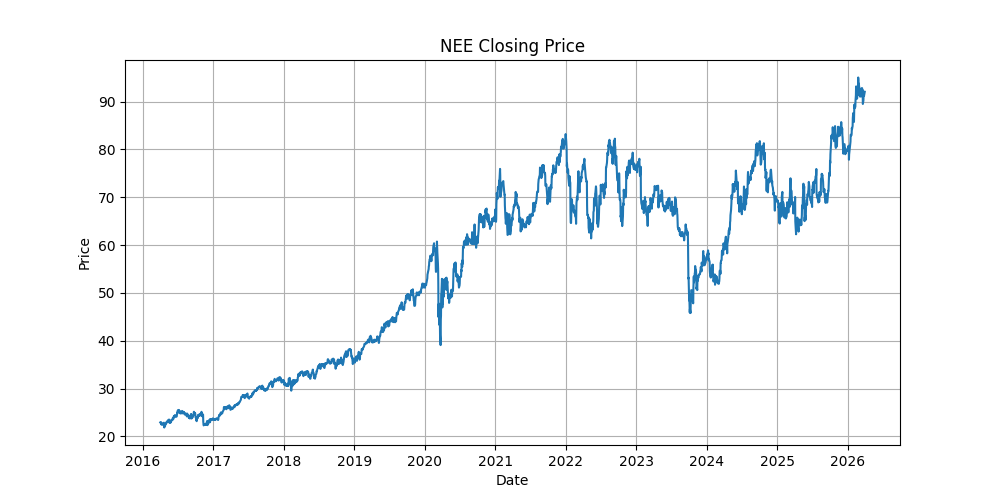
\includegraphics[width=\textwidth]{./images/NEE_data_presentation.png}
                \caption{Prezzo di chiusura}
            \end{subfigure}
        \end{figure}
    \item \textbf{Tesla (TSLA)}: 
        Il titolo mostra grandi picchi e grandi cali, ma ciò nonostante è in crescita rispetto all'inizio del periodo considerato.
        \begin{figure}[H]
            \centering
            \begin{subfigure}{0.43\textwidth}
                \centering
                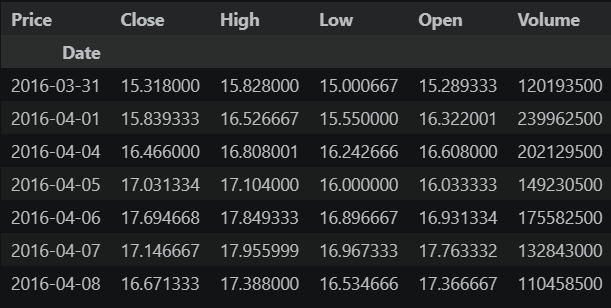
\includegraphics[width=\textwidth]{./images/TSLA_data_display.png}
                \caption{\texttt{DataFrame.head()}}
            \end{subfigure}
            \quad
            \begin{subfigure}{0.43\textwidth}
                \centering
                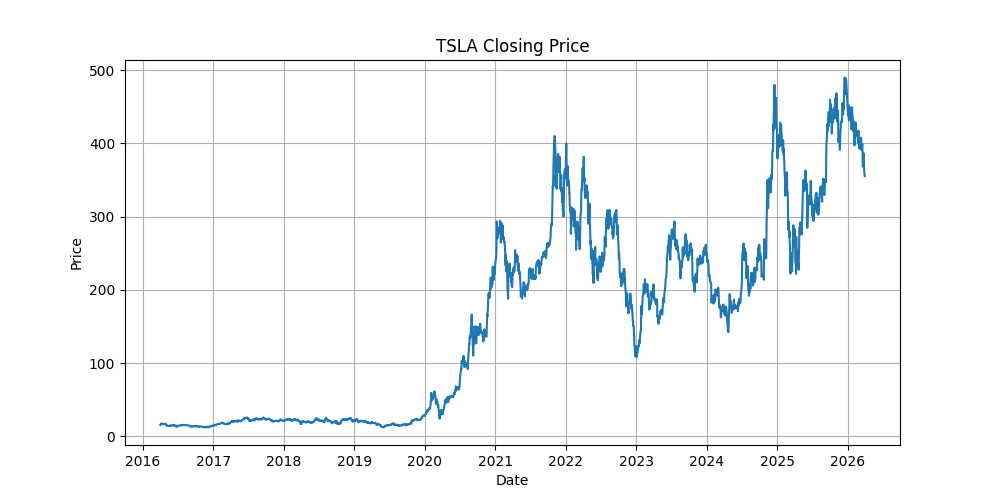
\includegraphics[width=\textwidth]{./images/TSLA_data_presentation.png}
                \caption{Prezzo di chiusura}
            \end{subfigure}
        \end{figure}
    \item \textbf{General Motors (GM)}: 
        Il titolo mostra un periodo di forte crescita soprattutto negli ultimi anni.
        \begin{figure}[H]
            \centering
            \begin{subfigure}{0.43\textwidth}
                \centering
                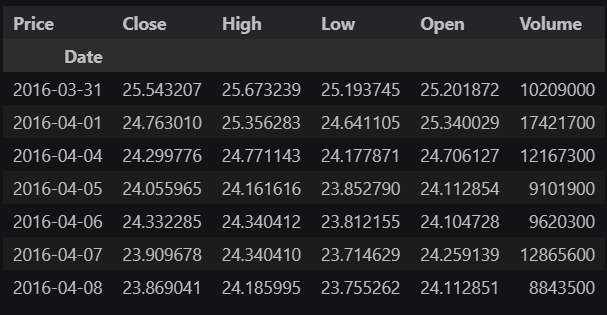
\includegraphics[width=\textwidth]{./images/GM_data_display.png}
                \caption{\texttt{DataFrame.head()}}
            \end{subfigure}
            \quad 
            \begin{subfigure}{0.43\textwidth}
                \centering
                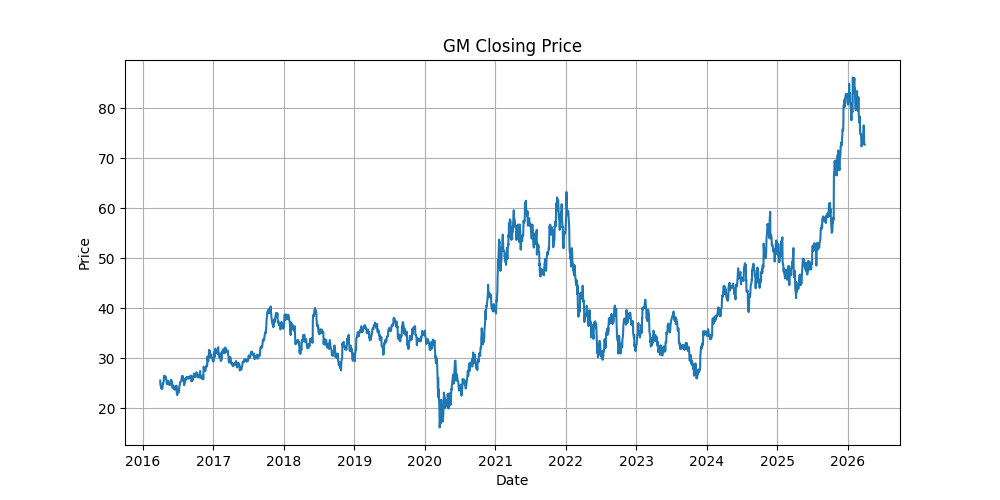
\includegraphics[width=\textwidth]{./images/GM_data_presentation.png}
                \caption{Prezzo di chiusura}
            \end{subfigure}
        \end{figure}
\end{itemize}

\chapter{Analisi Statistica}
\section{Rendimenti}
Per tutti i titoli presi in considerazione si può affermare che i rispettivi grafici oscillano costantemente attorno a una media che si colloca vicina allo zero.
Inoltre, è possibile notare lo shock di inizio 2020, dovuto alla pandemia, che ha portato a una forte volatilità, con rendimenti estremamente negativi in un breve periodo di tempo, ma anche picchi di rendimenti positivi.


\subsection{Settore tecnologico}
Un analisi visiva dei grafici dei titoli di Nvidia e Microsoft mostra una correlazione positiva visto che l'andamento dei rendimenti è quasi simile, con la sola differenza che Nvidia mostra un numero di picchi di rendimenti, sia positivi che negativi, maggiore.
Alcuni esempi sono:
\begin{itemize}
    \item Fine 2016: L'azienda smette di essere considerata solo come un produttore di schede grafiche per videogiochi e inizia a essere vista come in un ruolo chiave nell'addestratemento dell'intelligenza artificiale, dovuto al vantaggio delle GPU, rispetto alle CPU nella capacità computazionale.
    \item Fine 2018: Con il crollo delle criptovalute, subisce un forte calo a causa della diminuzione della domanda di GPU per il mining.
    \item Metà 2023: Riconducibile al picco di euforia dell'AI.
    \item inizio 2025: Un picco negativo dovuto all'uscita del modello cinese Deepseek, che riusciva ad avere prestazioni simili a quelle dei modelli di OpenAI, ma con un costo di addestramento molto più basso, quindi a un minor necessità di utilizzo di grandi quantità di GPU.
\end{itemize} 
\begin{figure}[H]
    \centering
    \begin{subfigure}{0.45\textwidth}
        \centering
        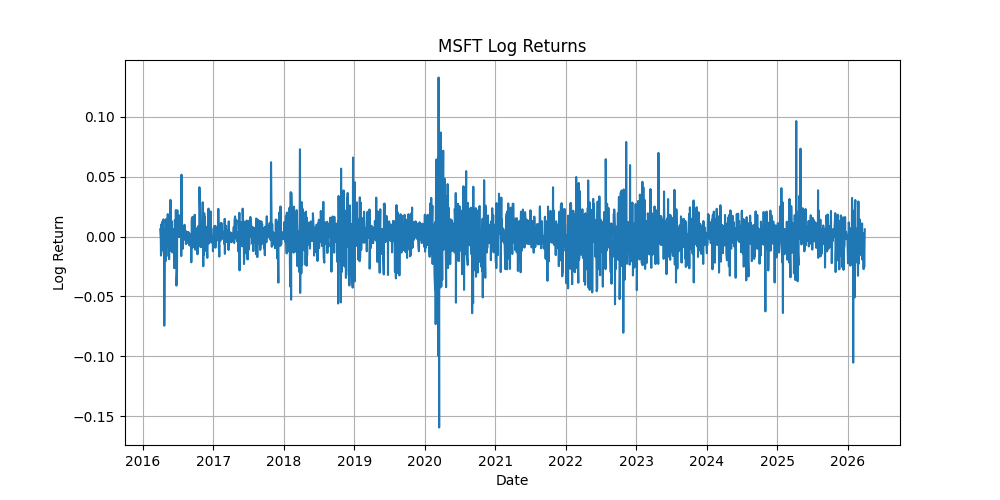
\includegraphics[width=\textwidth]{./images/MSFT_log_returns.png}
        \caption{Microsoft (MSFT)}
    \end{subfigure}
    \begin{subfigure}{0.45\textwidth}
        \centering
        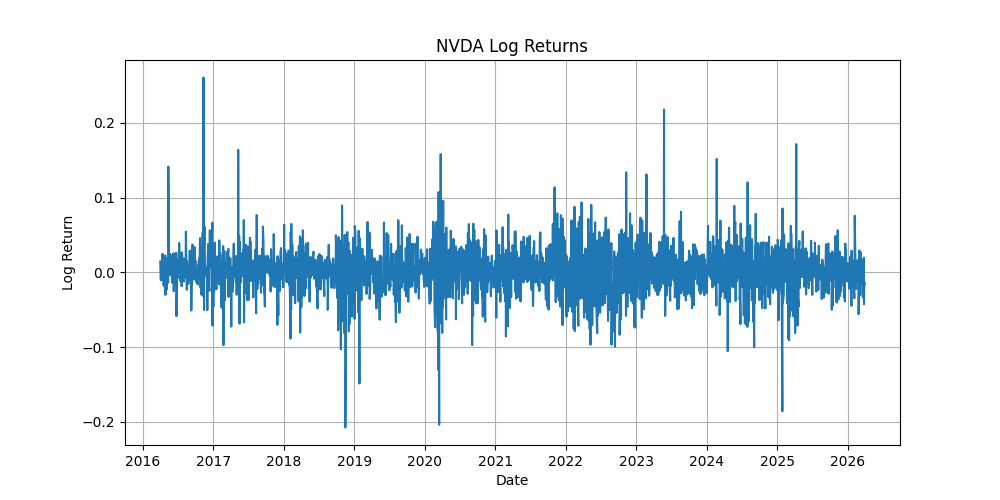
\includegraphics[width=\textwidth]{./images/NVDA_log_returns.png}
        \caption{NVIDIA (NVDA)}
    \end{subfigure}
\end{figure}
\subsection{Settore energetico}
Per quanto riguarda il settore energetico è possibile notare come entrambi i titoli siano più volatili nel periodo post pandemia rispetto al periodo precedente e specificatamente i rendimenti di ExxonMobil (XOM) siano più volatili rispetto a quelli di NextEra Energy (NEE), con picchi più pronunciati sia in positivo che in negativo. Questo potrebbe essere dovuto alla maggiore esposizione di ExxonMobil alle fluttuazioni dei prezzi del petrolio e alle tensioni geopolitiche, mentre NextEra Energy, essendo più orientata verso le energie rinnovabili, potrebbe essere meno influenzata da questi fattori.

Si può affermare perciò che questi due titoli hanno una correlazione positiva.

Uno dei picchi più rilevanti, diversi da quelli dovuti alla pandemia, è:
\begin{itemize}
    \item fine 2020: dovuto alla ripresa della domanda di petrolio dopo il crollo causato dalla pandemia, che ha portato a un aumento dei prezzi del petrolio.
\end{itemize}
\begin{figure}[H]
    \centering
    \begin{subfigure}{0.45\textwidth}
        \centering
        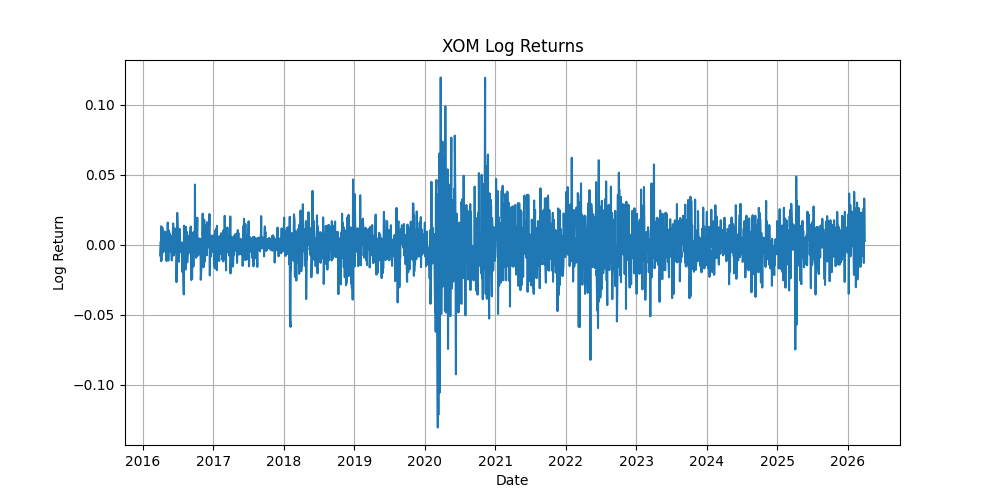
\includegraphics[width=\textwidth]{./images/XOM_log_returns.png}
        \caption{ExxonMobil (XOM)}
    \end{subfigure}
    \begin{subfigure}{0.45\textwidth}
        \centering
        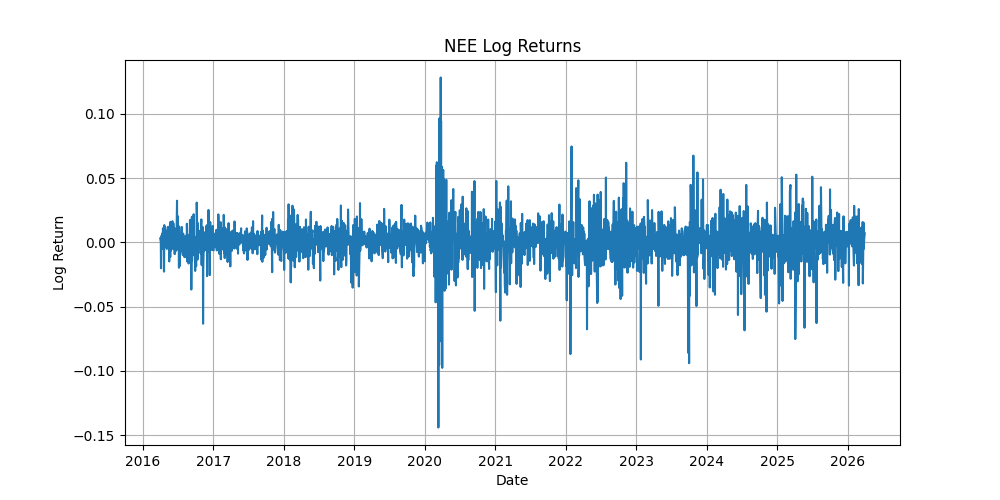
\includegraphics[width=\textwidth]{./images/NEE_log_returns.png}
        \caption{NextEra Energy (NEE)}
    \end{subfigure}
\end{figure}
\subsection{Settore automobilistico}
Nel settore automobilistico, invece, si evidenza che i due titoli presi in considerazione non mostrano una correlazione molto positiva e questo è dovuto al fatto che Tesla sia un'azienda influenzabile oltre che dal settore automobilistico, anche da quello tecnologico, visto gli investimenti nell'AI per lo sviluppo di macchine a guida autonoma, dal settore energetico, visto lo sviluppo di pannelli solari e dalle dichiarazione del CEO Elon Musk.
Alcuni esempi sono:
\begin{itemize}
    \item fine 2020: l'annuncio dell'esclusione di Tesla dall'indice S\&P 500.
    \item fine 2024: dovuto alla pubblicazione di bilanci che hanno sorpreso positivamente gli investitori, con un aumento dei ricavi e degli utili superiore alle aspettative.
    \item inizio 2025: causato da speculazioni sulla deregolamentazione riguardante i robotaxi che avrebbe favorito il lancio di questo servizio da parte di Tesla.
\end{itemize}
\begin{figure}[H]
    \centering
    \begin{subfigure}{0.45\textwidth}
        \centering
        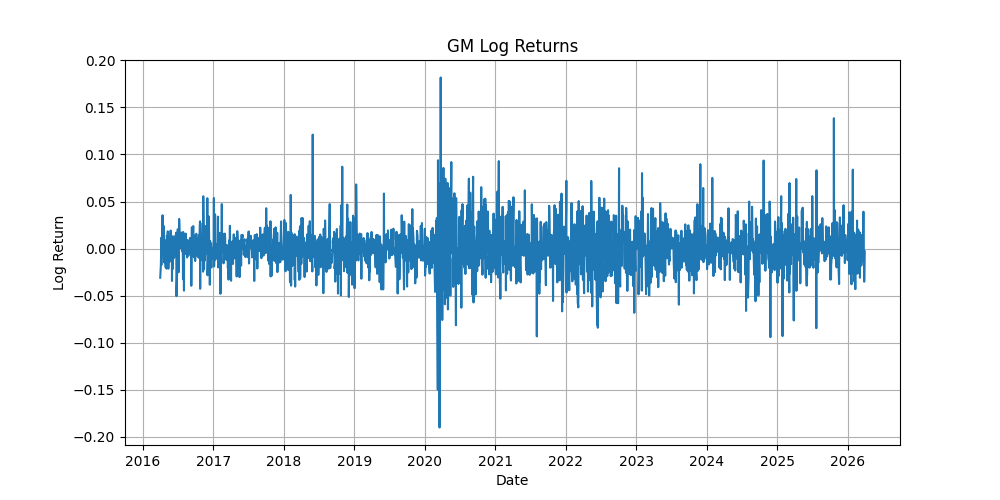
\includegraphics[width=\textwidth]{./images/GM_log_returns.png}
        \caption{General Motors (GM)}
    \end{subfigure}
    \begin{subfigure}{0.45\textwidth}
        \centering
        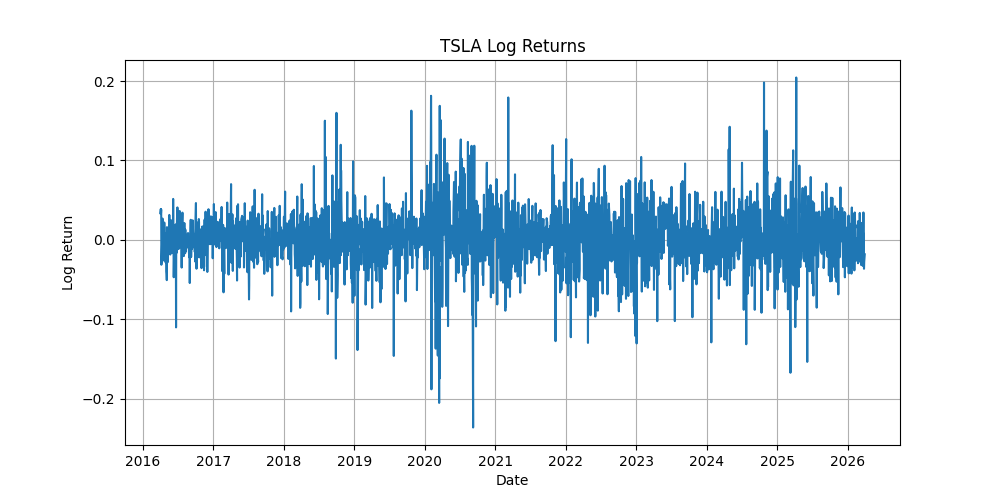
\includegraphics[width=\textwidth]{./images/TSLA_log_returns.png}
        \caption{Tesla (TSLA)}
    \end{subfigure}
\end{figure}

\section{Statistiche Descrittive}



\chapter{Previsione}

\section{Modello ARIMA}

\section{Strategie di Trading e Backtesting}

\section{Analisi Statica}

\section{Strategie Dinamiche}

\chapter{CAPM}

\chapter{Costruzione Portafoglio}

\end{document}
